
\chapter{线性代数}

线性代数是数学的一个分之,它主要处理线性关系问题,即数学对象之间的关系以一次形式表达的,它的主要研究对象为张量(tensor)即张量空间。


\section{标量,向量,矩阵和张量}

\subsection{标量}

单个数就是标量,比如3,5等。

\subsection{向量}

一组数就是向量,比如
\begin{equation}
  \begin{bmatrix}
    1 \\
    2 \\
    5 \\
    3
  \end{bmatrix}
\end{equation}

\subsection{矩阵}

矩阵就是2维数组,每个元素使用两个索引表示,比如
\begin{equation}
  \begin{bmatrix}
    A_{1,1} & A_{1,2} \\
    A_{2,1} & A_{2,2}
  \end{bmatrix}
\end{equation}

$A_{1,1}$ 表示矩阵中的第一行和第一列处的元素。

\subsection{张量}

当需要大于两个的数组表示的时候,就是张量,张量中的元素需要用$\ge 2$的索引来表示。


\begin{figure}[!ht]
  \centering
  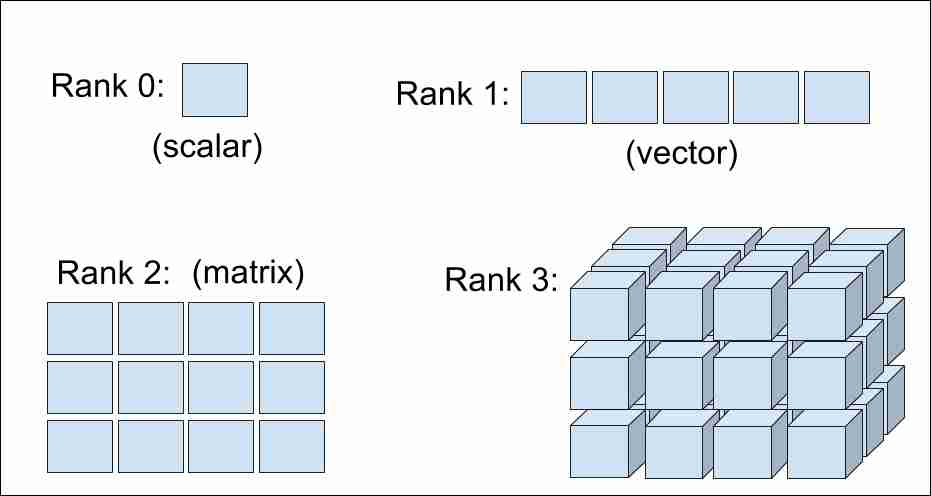
\includegraphics[width=\textwidth]{svmt.jpeg}
  \caption{标量,向量,矩阵和张量}
  \label{fig:svmt}
\end{figure}

\subsection{转置 (transpose)}

转置是矩阵的一种运算,即更换行和列。
我们用$A^\top$来表示矩阵$A$的转置,则
\begin{equation}
  (\bm{A}^\top)_{i,j} = A_{j,i}
\end{equation}


向量可以看作为只含有一列的矩阵,向量的转置是只含有一行的矩阵。

标量可以当作只含有一个元素的矩阵,因此,标量的矩阵就是标量本身。


\subsection{矩阵加法}

\begin{equation}
  \bm{C = A + B}
\end{equation}
这里 $C_{i,j} = A_{i,j} + B_{i,j}$,即如果两个矩阵的形状相同,矩阵的加法就是将对应索引的元素进行相加。


\subsection{矩阵的与标量的运算}

矩阵和一个标量进行相乘,相当于标量乘矩阵的所有元素,矩阵和标量相加,相当于矩阵中的所有元素都加该标量,即
\begin{equation}
  \bm{D} = a \cdot \bm{B} + c
\end{equation}
这里$D_{i,j} = a \cdot B_{i,j} + c$。

\subsection{矩阵与向量的运算}

在深度学习中,我们常常使用更简化的表示方式,允许将一个矩阵和一个向量进行相加,即
\begin{equation}
  \bm{C = A + b}
\end{equation}
这里$C_{i,j} = A_{i,j} + b_j$,即向量$b$被加到了矩阵的所有的列。

\section{矩阵乘法}

矩阵$\bm{A}$与矩阵$\bm{B}$相乘的前提是,$\bm{A}$的列数与$\bm{B}$的行数要相同。
假设$\bm{A}$的形状为$m\times n$,$\bm{B}$的形状为$n\times p$,那么$\bm{C}$的形状则为$m\times p$。
\begin{equation}
  \bm{C} = \bm{AB}
\end{equation}
这里
\begin{equation}
  C_{i,j} = \sum_k A_{i,k}B_{k,j}
\end{equation}
换句话说,$\bm{A}$的第$i$行乘$\bm{B}$的第$j$列,相乘的结果相加,得到$\bm{C}$的索引为$(i,j)$的元素。


\subsection{分配律(distributive)}

\begin{equation}
  \bm{A(B+C) = AB + AC}
\end{equation}

\subsection{结合律(associative)}

\begin{equation}
  \bm{A(BC) = (AB)C}
\end{equation}

\subsection{交换律(commutative)}

矩阵乘法不满足交换律。


\subsection{矩阵乘法的转置}

\begin{equation}
  \bm{(AB)^\top = B^\top A^\top}
\end{equation}

\section{线性方程的矩阵表达}

假设有如下线性方程组:
\begin{equation}
  \label{eq:linear-equation}
  \begin{cases}
    a_{1,1}x_1 + a_{1,2}x_2 + \cdots + a_{1,n}x_n  =  b_1 \\
    a_{2,1}x_1 + a_{2,2}x_2 + \cdots + a_{2,n}x_n  =  b_2 \\
    \quad \quad \quad \quad \quad \cdots  \\ 
    a_{m,1}x_1 + a_{m,2}x_2 + \cdots + a_{m,n}x_n  =  b_m
  \end{cases}
\end{equation}

线性方程组中,所有的系数$a$组成一个矩阵$\bm{A}$:
\begin{equation}
  \bm{A} =
  \begin{bmatrix}
    a_{1,1} & a_{1,2} & \cdots & a_{1,n} \\
    a_{2,1} & a_{2,2} & \cdots & a_{2,n} \\
    & & \cdots \\
    a_{m,1} & a_{m,2} & \cdots & a_{m,n} \\
  \end{bmatrix}
\end{equation}
方程组中所有等号右边的数组成一个向量$\bm{b}$:
\begin{equation}
  \bm{b} =
  \begin{bmatrix}
    b_1 \\
    b_2 \\
    \cdots \\
    b_n
  \end{bmatrix}
\end{equation}

所有的待求系数$x$组成向量$\bm{x}$:
\begin{equation}
  \bm{x} =
  \begin{bmatrix}
    x_1 \\
    x_2 \\
    \cdots \\
    x_n
  \end{bmatrix}
\end{equation}

根据矩阵乘法定义,则线性方程组可以写为:
\begin{equation}
  \label{eq:linear-equation-vector}
  \bm{Ax} = \bm{b}
\end{equation}








\section{单位矩阵(identity matrix)}

单位矩阵就是,当单位矩阵和一个向量相乘时,结果还是该向量本身,即
\begin{equation}
  \forall \bm{x} \in \mathbb{R}^n, \bm{I}_n = \bm{x}.
\end{equation}

有定义可知,单位矩阵主对角线上的元素都为1,其余都为0,如:
\begin{equation}
  \begin{bmatrix}
    1 & 0 & 0 \\
    0 & 1 & 0 \\
    0 & 0 & 1
  \end{bmatrix}
\end{equation}
表示$\bm{I}_3$。

\section{逆矩阵(inverse matrix)}

我们用$\bm{A}^{-1}$来表示矩阵$\bm{A}$的逆矩阵,定义如下:
\begin{equation}
  \bm{A}^{-1}\bm{A} = \bm{I}_n
\end{equation}


\section{扩张空间(span)}
对于\eqref{eq:linear-equation-vector}所示的矩阵表达的线性方程组的解,
将矩阵$\bm{A}$的每一列当作一个向量,表示从原点指向特定的方向,
则方程组的解的个数表示有多少种方式到达$\bm{b}$。
从这个观点来看,$\bm{x}$的每个元素表示在每个方向上走多远,
$x_i$表示在$i$列方向上走多远:
\begin{equation}
  \label{eq:linear-combination}
  \bm{Ax} = \sum_i x_i \bm{A}_{:,i}.
\end{equation}

\eqref{eq:linear-combination}表示的操作称为“线性组合”。

正式的,一组向量集 $\{v^{(1)},... , v^{(n)}\}$ 的线性组合通过将每一个向量乘一个标量得到:
\begin{equation}
  \sum_i c_i \bm{v}^{(i)}
\end{equation}

一组向量的“扩展空间”是通过对该组向量的线性组合而可以达到的所有点的集合。




\section{线性相关,线性无关}

对于一组向量组成的集合,如果集合中的任一向量都无法用其余向量的线性组合进行表示,
则该组向量是线性无关的,否则为线性相关的。


\section{模}

在机器学习中,我们用模(norm)来表示向量的大小。

常用的$L^p$模定义如下:
\begin{equation}
  \label{eq:lp}
  ||\bm{x}||_p = \left ( \sum_i |x_i|^p \right )^{\frac{1}{p}}
\end{equation}
对$p\in \mathbb{R}, p>1$。


模,包括$L^p$模,是这样一类函数,映射向量到非负数。
更严格的讲,模函数需要满足如下特性:
\begin{itemize}
\item $f(x) = 0 \Rightarrow x=0$
\item $f(x+y) \le f(x) + f(y)$
\item $\forall \alpha \in \mathbb{R}, f(\alpha x)=|\alpha|f(x)$
\end{itemize}

其中$L^2$模也常称为欧式模。


机器学习中常用的一个模为$L^\infty$模,也叫最大模:
\begin{equation}
  \label{eq:max-norm}
  ||\bm{x}||_\infty = \max_i |x_i|.
\end{equation}


深度学习中,我们有时希望测量矩阵的大小,常用Frobenius模来表示:
\begin{equation}
||A ||_F=\sqrt{\sum_{i,j}A_{i,j}^2}
\end{equation}


\section{对称矩阵}

对阵矩阵(symmetric matrix),顾名思义,就是转置矩阵等于本身的矩阵:
\begin{equation}
  \bm{A} = \bm{A}^\top
\end{equation}

例如:
\begin{equation}
  \begin{bmatrix}
    1 & 2 & 3 \\
    2 & 4 & 5 \\
    3 & 5 & 6
  \end{bmatrix}
\end{equation}

\section{正交矩阵(orthogonal matrix)}

单位向量就是模为1的向量:
\begin{equation}
  ||\bm{x}||_2 = 1.
\end{equation}


如果满足$\bm{x}^\top\bm{y}$,则我们说向量$\bm{x}$和向量$\bm{y}$相互正交。

如果向量不仅正交,而且模等于1,则称它们为标准正交的。


正交矩阵为这样的矩阵,它的行是相互标准正交的,它的列也是相互标准正交的:
\begin{equation}
  \label{eq:orthogonal-matrix}
  \bm{A}^\top \bm{A} = \bm{AA}^\top = \bm{I}
\end{equation}

因此可知:
\begin{equation}
  \bm{A}^{-1} = \bm{A}^\top
\end{equation}

\section{特征分解}

为什么要进行矩阵分解?

将数学物体(mathematical object)分解成组成要素,而不仅仅是它原始的表现形式,
有时候方便我们更好的理解它们或者发现它们通用的特性。
比如:
12这个数字,如果用十进制表示,则为12,
如果用2进制表示,则为1100,
如果用16进制表示,则为C,
但是,12可以分解为$12 = 2\times 2 \times 3$却总是真的,
因而我们可以知道,12可以被2整除,不能被5整除。
矩阵分解就类似于数的因式分解,
通过对矩阵进行矩阵分解,
我们可以更好的理解矩阵的特性。


\begin{tcolorbox}
  mathematical object,我不喜欢用数学对象来表述,而更喜欢用数学物体,
  这个物体是一种统称,而不仅仅是现实生活中的一种实物,
  数学符号也是一种数学物体,
\end{tcolorbox}

使用最广泛的矩阵分解为特征值分解(eigendecomposition),即将矩阵分解为一组特征向量和特征值。
方阵$\bm{A}$的特征向量为非零向量$\bm{v}$满足:
\begin{equation}
  \label{eq:eigendefunction}
  \bm{Av} = \lambda \bm{v}.
\end{equation}
标量$\lambda$为特征向量对应的特征值。

假设矩阵$\bm{A}$有$n$个线性无关的的特征向量$\{\bm{v}^{(1)}, ..., \bm{v}^{(n)}\}$,
对应的特征值为$\{\lambda_1, ... , \lambda_n\}$,
将所有的特征向量组成矩阵$\bm{V} = [\bm{v}^{(1)}, ..., \bm{v}^{(n)}]$,
将所有的特征值组成向量$\bm{\lambda} = [\lambda_1, ... , \lambda_n]$,
则$\bm{A}$的特征分解为:
\begin{equation}
  \label{eq:eigendecomposition}
  \bm{A} = \bm{V}\text{diag}(\lambda)\bm{V}^{-1}
\end{equation}

\subsection{正定矩阵}

如果一个矩阵的所有特征值都为正数,则该矩阵为“正定矩阵”。

\begin{tcolorbox}
  \begin{equation}
    \bm{Av} = \lambda\bm{v} 
  \end{equation}
  \begin{equation*}
    \Downarrow
  \end{equation*}
  \begin{equation}
    \begin{cases}
      \bm{Av}_1 = \lambda_1\bm{v}_1 \\
      \cdots \\
      \bm{Av}_n = \lambda_n\bm{v}_n \\
    \end{cases}
  \end{equation}
  \begin{equation*}
    \Downarrow
  \end{equation*}
  \begin{equation}
    \bm{A}[\bm{v}_1,\dots,\bm{v}_n] = [\lambda_1\bm{v}_1, \dots, \lambda_n\bm{v}_n]
  \end{equation}
  \begin{equation*}
    \Downarrow
  \end{equation*}
  \begin{equation}
    \bm{A}[\bm{v}_1,\dots,\bm{v}_n] = [\bm{v}_1,\dots,\bm{v}_n]
    \begin{bmatrix}
      \lambda_1 & \dots & 0 \\
      & \vdots & \\
      0 & \dots & \lambda_n
    \end{bmatrix}
  \end{equation}
  令$\bm{V} = [\bm{v}_1,\dots,\bm{v}_n]$,
  $\bm{\lambda} = [\lambda_1, ... , \lambda_n]$,
  则:
  \begin{equation}
    \bm{AV} = \bm{V}\text{diag}(\lambda)
  \end{equation}
  \begin{equation*}
    \bm{A} = \bm{V}\text{diag}(\lambda)\bm{V}^{-1}
  \end{equation*}
\end{tcolorbox}

\section{奇异值分解(singular value decompositon)}
奇异值分解可以提供给我们特征值分解相同的信息,但其应用更广泛,因为可以使用奇异值分解的矩阵的范围更广,
比如,如果矩阵中的元素都是实数,该矩阵不是方阵,则不用使用特征值分解,但却可是使用奇异值分解。
任一实数矩阵都有对应的奇异值分解。


假设矩阵$\bm{A}$的形状为$m\times n$,则
\begin{equation}
  \label{eq:svd}
  \bm{A=UDV}^\top
\end{equation}
$\bm{U}$为$m\times m$的正交矩阵,
$\bm{D}$为$m\times n$的对角矩阵,
$\bm{V}$为$n\times n$的正交矩阵。

